\section{課題3}
課題3のソースコードと実行結果を示す.


\subsection{課題3-1}
\lstinputlisting[caption=kadai3-1.py]{../source/kadai3-1.py}

\subsection{課題3-2}
\lstinputlisting[caption=kadai3-2.py]{../source/kadai3-2.py}

実行結果は以下のようになった.

\begin{figure}[h]
  \begin{center}
    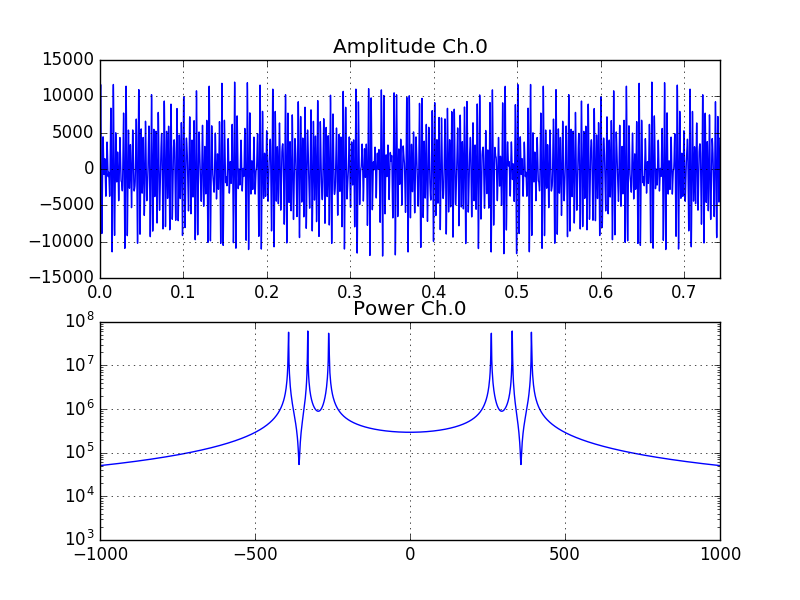
\includegraphics[width=10cm]{./img/kadai3-2.png}
    \caption{課題3-2}
  \end{center}
\end{figure}

上の波形により3つの波が合成されていることが分かる.また,下のスペクトルより262,330,393Hzの部分が大きく出ていることが確認できる.

よって,C,E,Gの3音による和音が出力されたと言える.
